\section{结果}
\label{sec:results}

\subsection{准确率低于平凡上限，判别力处于随机水平}
\label{sec:results-accuracy}

在 NIH 干净单元上，七个病理标签（七个全阴；排除 \texttt{no\_finding}）的多数类上限为标签槽位的 \textbf{0.6579}。没有模型超过该上限 1.0\,\pp{} 以上；最好的 InternVL3.5（0.6674）为 +0.95\,\pp{}，Qwen2.5-VL（0.6578）甚至\emph{低于}上限。所有模型的干净 AUROC 为 0.50--0.63（表~\ref{tab:clean}）。以准确率优先的报告会把这张表描述为``0.54--0.67 的准确率''；加入上限后，同一张表说明的是``任何地方都没有可用的判别力''。该主张的监督复现在第~\ref{sec:results-baseline} 节。

\begin{table}[t]
\centering
\small
\caption{NIH 干净性能与七病理标签上的全阴上限（排除 \texttt{no\_finding}；$n=1{,}506$ 例研究，10,542 个病理槽位）。上限在每个模型的确定槽位上计算：0.6579；CheXagent 为 0.6570，因为它只有 18.9\% 的槽位具有确定状态。宏 AUROC 为七个病理标签上的患者聚类自助法 95\% 区间（1,000 次重采样；缺失概率按 0.0 计，与脚本 75 一致）。}
\label{tab:clean}
\begin{tabular}{lrrrrr}
\toprule
模型 & 合并准确率 & 相对上限 & 宏平均 AUROC [95\% CI] & 宏平均 ECE & 阳性召回率 \\
\midrule
InternVL3.5 & 0.6674 & $+1.0$\,\pp{} & 0.6066 [0.5949, 0.6191] & 0.247 & 0.4928 \\
MedGemma-1.5 & 0.6106 & $-4.7$\,\pp{} & 0.5852 [0.5748, 0.5952] & 0.234 & \textbf{0.6392} \\
MedGemma-4B & 0.5398 & $-11.8$\,\pp{} & 0.6270 [0.6138, 0.6394] & 0.207 & 0.5519 \\
Qwen3-VL & 0.5926 & $-6.5$\,\pp{} & 0.5455 [0.5350, 0.5568] & 0.348 & 0.1625 \\
Qwen2.5-VL & 0.6578 & $\mathbf{-0.01}$\,\pp{} & 0.5013 [0.5003, 0.5027] & 0.412 & 0.0039 \\
CheXagent & 0.0589 & $-59.8$\,\pp{} & 0.5001 [0.5000, 0.5002] & 0.310 & 0.0003 \\
\bottomrule
\end{tabular}
\end{table}

宏 ECE 作为描述性的可靠性摘要报告，而不是校准主张：概率以文字形式写在回答里，只对确定槽位存在，CheXagent 根本没有概率通道，也未做任何事后校准。因此本表中只有 AUROC 一列是六个模型间可比的判别量。

\subsection{退化可以通过移动工作点提高召回率}
\label{sec:results-op}

表~\ref{tab:op} 报告合并层面的重度对干净变化。工作点案例是那些干净阳性预测率较高的模型；基线很低的模型没有向上移动的空间。这是\emph{测量体制}的性质，而不是``退化无害''的主张：两个 InternVL3.5 行的精确率下降（$-1.38$ 与 $-0.64$\,\pp{}），Qwen3-VL 的精确率略升（$+0.19$\,\pp{}），而三个单元的阳性预测率都上升，假阳性分别增加 16\%、8\% 与 20\%。InternVL3.5 对比度单元的增加集中在肺炎（$+98$）与实变（$+69$），占 259 例新增假阳性的 64.5\%，气胸为 0（表~\ref{tab:flip}）。患者聚类自助法（1,000 次重采样；\url{scripts/85_operating_point_ci.py}）给出三个单元的 $\Delta$召回率：$+4.69$ $[3.75,5.56]$、$+2.52$ $[1.46,3.63]$、$+3.44$ $[2.37,4.69]$\,\pp{}；$\Delta$阳性预测率：$+4.06$ $[3.44,4.64]$、$+2.09$ $[1.36,2.85]$、$+2.51$ $[1.75,3.26]$；所有区间都排除零。精确率变化只有 InternVL3.5 对比度单元排除零（$-1.38$ $[-2.16,-0.63]$\,\pp{}）；另外两个区间包含零。对 InternVL3.5 对比度单元，病例级转移（附录~\ref{app:risk}，表~\ref{tab:flip}）显示的是广泛重分类，而不是有针对性地找回丢失发现；下文的固定规则重跑表明分数分布本身在移动，因此我们把该模式标记为\emph{工作点移动}，而不是已被证明的阈值变化。对输出的概率做事后固定 $0.5$ 切点，可复现同样的变化（对比度 $+4.80$ 对 $+4.69$\,\pp{}，亮度 $+2.47$ 对 $+2.52$\,\pp{}，Qwen3-VL $+3.36$ 对 $+3.44$\,\pp{}；附录~\ref{app:risk}，表~\ref{tab:fixedthr}），因此该移动不是离散状态规则改变造成的伪影。它仍是工作点移动，因为概率尺度本身发生了移动。真正的固定规则重跑确认了这一点：只要求模型输出概率、由我们在 0.5 处赋状态，对比度 severe 使召回由 0.510 升至 0.575、阳性率由 0.404 升至 0.449，亮度 severe 使召回升至 0.584、阳性率升至 0.457（200 例配对研究；附录~\ref{app:risk} 表~\ref{tab:fixedrerun}）。由于该运行的决策规则不可能移动，增益来自分数分布移动，而不是离散状态规则改变。第二个推理模型以相反方向复现了该工作点机制（第~\ref{sec:results-second} 节）。反转 3 也不需要语言模型：同一个 DenseNet-121 检查点在 19 格网格上以固定 0.5 规则运行，对比度 severe 下合并召回由 0.567 升至 0.588、阳性率由 0.360 升至 0.378，而宏 AUROC 保持 0.733 $\rightarrow$ 0.729；噪声 severe 使召回降至 0.477、阳性率降至 0.321，分辨率 severe 降至 0.523 与 0.355（附录~\ref{app:risk} 表~\ref{tab:densenetgrid}）。因此机制是分数分布在移动，而不是文字状态在移动；模型间不同的是移动幅度（InternVL3.5 为 +4.7\,\pp{}，DenseNet 为 +2.1\,\pp{}）。

\begin{table}[t]
\centering
\small
\caption{重度对干净，七个病理标签合并（$n=1{,}506$；10,542 个病理槽位）。}
\label{tab:op}
\begin{tabular}{llrrrrl}
\toprule
模型 & 退化 & $\Delta$ 召回 & $\Delta$ 精确率 & $\Delta$ 阳性率 & 假阳性 & 判定 \\
\midrule
InternVL3.5 & 对比度 & $\mathbf{+4.69}$\,\pp{} & $-1.38$\,\pp{} & $\mathbf{+4.06}$\,\pp{} & 1,646 $\rightarrow$ 1,905 & 工作点移动 \\
InternVL3.5 & 亮度 & $+2.52$\,\pp{} & $-0.64$\,\pp{} & $+2.09$\,\pp{} & 1,646 $\rightarrow$ 1,775 & 工作点移动 \\
Qwen3-VL & 对比度 & $+3.44$\,\pp{} & $+0.19$\,\pp{} & $+2.51$\,\pp{} & 696 $\rightarrow$ 837 & 工作点移动 \\
MedGemma-1.5 & 对比度 & $+0.78$\,\pp{} & $+0.20$\,\pp{} & $+0.36$\,\pp{} & 2,425 & 稳定 \\
MedGemma-4B & 对比度 & $-1.66$\,\pp{} & $-0.40$\,\pp{} & $-0.87$\,\pp{} & 2,168 & 稳定 \\
MedGemma-1.5 & 分辨率 & $\mathbf{-18.77}$\,\pp{} & $-1.43$\,\pp{} & $-12.21$\,\pp{} & 1,786 & 召回损失 \\
MedGemma-4B & 噪声 & $\mathbf{-22.99}$\,\pp{} & $-0.09$\,\pp{} & $-16.51$\,\pp{} & 1,288 & 召回损失 \\
\bottomrule
\end{tabular}
\end{table}

\subsection{两个可分离的轴：可察觉性与损伤}
\label{sec:results-twoaxis}

对 MedGemma-1.5，推理通道触发率（以 \texttt{<unused94>thought} 开头的回答）是我们的操作化、\emph{基于标记}的读数：它记录模型是否进入与``注意到退化图像''相关的推理模式，而不表示模型是否具有该退化的内部表征。在 19 格网格上，基于标记的可察觉性按退化类别分离，而损伤并不跟随它（表~\ref{tab:twoaxis}）。

\begin{table}[t]
\centering
\small
\caption{基于标记的可察觉性与损伤（MedGemma-1.5，重度）。损伤排名把干净单元记为第 1 名，再按带符号的召回变化排列六个重度退化（最有害者在前）；可察觉性排名按标记率排列六个重度退化（最高者在前）。该标记是模型侧信号，不是图像侧可见性的度量。}
\label{tab:twoaxis}
\begin{tabular}{lrrrr}
\toprule
退化 & 标记率（重度） & 重度 $\Delta$ 召回 & 损伤排名 & 可察觉性排名 \\
\midrule
分辨率 & \textbf{71.98\%} & $-18.77$\,\pp{} & 2 & 1 \\
噪声 & \textbf{0.46\%} & $-17.22$\,\pp{} & 3 & 5 \\
模糊 & 29.35\% & $-5.10$\,\pp{} & 5 & 2 \\
JPEG & 27.42\% & $-9.03$\,\pp{} & 4 & 3 \\
对比度 & 0.60\% & $+0.78$\,\pp{} & 7 & 4 \\
亮度 & 0.20\% & $-1.19$\,\pp{} & 6 & 6 \\
\bottomrule
\end{tabular}
\end{table}

可察觉性与损伤之间的秩相关不是重点；重点是\emph{非对角线}。对 MedGemma-1.5——矩阵中唯一具有可读推理通道的模型——噪声造成的损伤与分辨率损失相当（$-17.2$ 对 $-18.8$\,\pp{}），而标记触发率低 \textbf{156 倍}（0.46\% 对 71.98\%）。其余五个模型不暴露该通道，其标记率结构性为 0，因此我们不做跨模型标记平均，也不把双轴结果解释为跨模型证据。在这一单模型范围内，结果是\textbf{静默失效象限}（图~\ref{fig:silent}）：一种破坏证据却不触发模型自监控信号的退化。对于监视推理通道激活或 token 级犹豫的部署监控器，噪声是看不见的。

两个控制排除了伪影。第一，\texttt{marker\_unparsed}（模型打开了通道却未能闭合 JSON）在整个网格上 $\le 1.20\%$，因此标记不是截断的代理。第二，干净单元只有 0.13\% 的回答打开通道，因此标记并非无条件出现。

第三个控制把失效定位在模型侧而非图像侧。在 1,506 张域内评估图像上，单一无参考统计量（Laplacian 方差）把干净图像与重度噪声图像分开的 AUC 为 $1.000$；高频能量的中位数从 $0.0011$ 升至 $0.0844$（附录~\ref{app:risk}，表~\ref{tab:imageside}）。同一统计量以相反方向把干净图像与重度模糊图像分开，AUC 同样为 $1.000$。因此，退化对通用图像质量监控器而言一目了然；失效的是模型自身的自监控通道。这把主张收窄到我们真正辩护的那一条：模型的监控信号没有登记一种会损害其答案的退化。该轴对的跨模型检验见第~\ref{sec:results-second} 节。

第四个基于规则的检查问：模型是否会\emph{用文字}说出来，而不是通过标记。在原始回答中搜索显式质量词（noise、degraded、quality、artifact、blur），六个模型在重度噪声下均为 \textbf{0.00\%}；MedGemma-1.5 在重度分辨率下为 3.85\%（58/1,506）；其他模型在该单元均不超过 0.00\%（\url{scripts/83_quality_language_audit.py}）。低标记率并没有被显式语言补偿。

\begin{figure}[t]
\centering
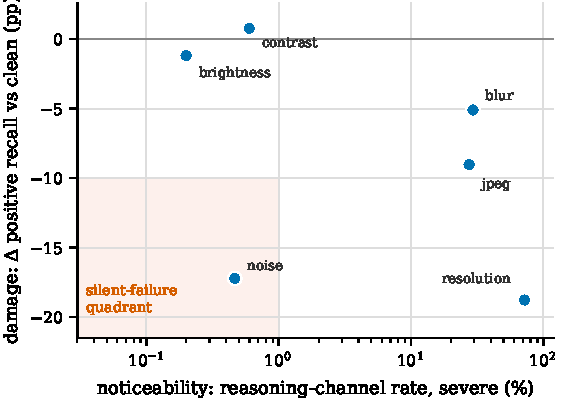
\includegraphics[width=0.62\textwidth]{figures/fig03_silent_failure.pdf}
\caption{静默失效象限（MedGemma-1.5，矩阵中唯一具有可读推理通道的模型）。基于标记的可察觉性是重度退化下的推理通道触发率；损伤是合并阳性召回的变化。阴影区域为低可察觉性且损伤显著；噪声落在其中。}
\label{fig:silent}
\end{figure}

\subsection{契约决定捷径的形式}
\label{sec:results-schema}

在模型、提示内容与空白图像固定的条件下，五种模式产生两种互不相交的失效形式（表~\ref{tab:schema}）。四种模式产生 \textbf{0/1,506} 条模式合规的空白回答，且都把 \texttt{no\_finding} 以概率 1.0 判为阳性。带 \texttt{uncertain} 状态的逐标签模式产生 \textbf{1,506/1,506} 条合规回答，75\% 的槽位弃答，\texttt{no\_finding} 阳性率为 0\%。两者的 Wilson 区间不重叠。

\begin{table}[t]
\centering
\small
\caption{模式消融，MedGemma-4B（每单元 $n=1{,}506$）。}
\label{tab:schema}
\begin{tabular}{lrrrr}
\toprule
模式 & 空白合规数 & 空白 \texttt{no\_finding} 阳性 & 真实召回 & 空白弃答率 \\
\midrule
v0 简单 & 0/1,506 & 1.000 & \textbf{0.499} & 0\% \\
v1 逐标签二分类 & \textbf{1,506/1,506} & 0.000 & 0.442 & \textbf{75\%} \\
v2 few-shot & 0/1,506 & 1.000 & 0.269 & 0\% \\
v3 报告优先 & 0/1,506 & 1.000 & 0.315（22.3\% 不可解析） & 0\% \\
v4 正常性压力 & 0/1,506 & 1.000 & \textbf{0.166} & 0\% \\
\bottomrule
\end{tabular}
\end{table}

同一实验反转了对提示敏感性的通常解读：产生最佳\emph{真实图像}召回的模式（v0），正是产生最自信\emph{空白图像}断言的那个模式。因此，``提示调优''与``grounding 诊断''不能互相替代。第二个医学模型上的复现与措辞对照见第~\ref{sec:results-schema2}~与~\ref{sec:results-paraphrase} 节。

\subsection{响应性在域外坍缩}
\label{sec:results-collapse}

表~\ref{tab:audit} 展示了坍缩；这里我们检验最明显的混杂。PadChest 的疾病阳性率低于 NIH（17.7\% 的研究至少含一个疾病标签，NIH 为 92.0\%；其余 NIH 研究仅含 no-finding），因此``永远回答正常''在 PadChest 上是更好的先验。限制到 \textbf{265 例疾病阳性研究}，六个模型中仍有五个坍缩：MedGemma-4B 8 种（众数 90.6\%）、InternVL3.5 2 种（89.4\%）、Qwen3-VL 2 种（99.6\%）、CheXagent 2 种（95.5\%）、Qwen2.5-VL 1 种（100\%）；只有 MedGemma-1.5 保持 91 种（34.7\%）。一个对其疾病阳性研究只给出一种回答的模型不是``保守''，而是没有响应性，其空白对照不可识别（图~\ref{fig:resp}）。这也解释了跨数据集迁移结果：常数函数按构造 AUROC 为 0.5。两个观察是同一事实的两次呈现。

\textbf{第七个模型：只在散文层运行。}LLaVA-Med 在 PadChest、Open-i 与一个 200 例 NIH 子集上运行，未跑完整的 28,614 单元网格，因为该子集已经显示同样的常数模板。它是一个\emph{双模板}模型：在 1,500 例 PadChest 研究上给出 19 种不同回答，其中 59.1\% 为同一模板、23.3\% 为空字符串、2.1\% 为安全免责声明；其 PadChest 空白回答 100\% 为空。在 Open-i 上它只给出两种回答：67.05\% 为``该胸片似乎无法判读''，32.95\% 为一句固定正常描述，任何研究都没有发现级内容。在 NIH 子集上它同样只给出两种回答，其中一种占 98.7\%，结构化解析率为 0\%，空白回答为空。因此，我们把它报告为\emph{实测}排除，而不是设计排除，并且不在发现层面给它打分（表~\ref{tab:audit}）。

\begin{figure}[t]
\centering
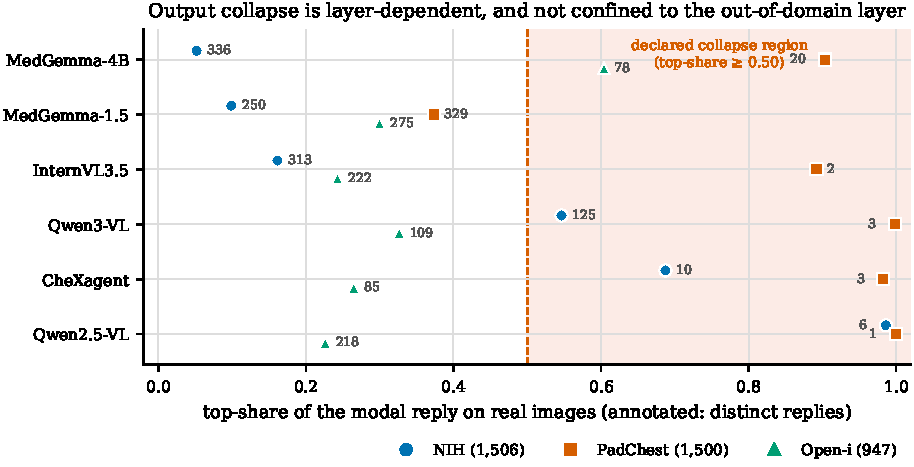
\includegraphics[width=\textwidth]{figures/fig02_responsiveness.pdf}
\caption{三个数据层上的响应性。每个标记是真实图像上众数回答的占比；旁边的数字是不同回答的数量。阴影区域是预先声明的坍缩规则。}
\label{fig:resp}
\end{figure}

\subsection{没有零模型的空白对照不是依赖度量}
\label{sec:results-null}

每个模型的空白回答都坍缩到极小的模板集合——五个模型为 1--2 种，Qwen2.5-VL 为 11 种样板变体，其中众数变体占 39.7\%。对 Qwen3-VL 与 CheXagent，该模板是\textbf{拒答}（``该研究无法判读……''，分别占空白回答的 96.3\% 与 100\%）；对其他四个模型，它是\textbf{通用正常报告}。在每种情况下，正确的零点是真实图像间相似度，而不是零相似度（表~\ref{tab:blanknull}，图~\ref{fig:null}）。

\begin{table}[t]
\centering
\small
\caption{Open-i 空白对照及其真实图像间零模型（$n=947$）。$\Delta_{\text{null}} = J(\text{真实},\text{另一真实}) - J(\text{真实},\text{空白})$ 即第~\ref{sec:preconditions}~节的距离型分离：正值表示空白回答比随机真实回答离真实回答更远。}
\label{tab:blanknull}
\begin{tabular}{lrrrl}
\toprule
模型 & $J(\text{真实},\text{空白})$ & $J(\text{真实},\text{另一真实})$ & $\Delta_{\text{null}}$ & 空白模板 \\
\midrule
CheXagent & 0.277 & 0.247 & $-0.030$ & 拒答 \\
Qwen3-VL & 0.091 & 0.740 & $+0.648$ & 拒答 \\
Qwen2.5-VL & 0.576 & 0.770 & $+0.193$ & 第二样板 \\
InternVL3.5 & 0.562 & 0.673 & $+0.112$ & 通用正常 \\
MedGemma-1.5 & 0.736 & 0.648 & $-0.087$ & 通用正常 \\
MedGemma-4B & 0.894 & 0.824 & $-0.070$ & 通用正常 \\
\bottomrule
\end{tabular}
\end{table}

原始 Jaccard 所暗示的排序（Qwen3-VL 最 grounded，MedGemma-4B 最差）在检查模板后不成立。最纯粹的案例是 LLaVA-Med：其 67.05\% 的真实 Open-i 回答与空白拒答逐字节相同，其余 32.95\% 是一句正常描述——两个模板，没有发现。PadChest 上的坍缩不是空字符串造成的伪影：只看 1,150 条非空回答，仍有 18 种不同字符串，众数占 77.0\%。结构化层同样如此：六个模型的空白回答都坍缩为一个 JSON 模板。概率空间分离是唯一能区分结构化模型的统计量，而且只区分三个：MedGemma-4B（NIH $+0.131$）、InternVL3.5（NIH $+0.041$）、MedGemma-1.5（PadChest $+0.134$）。对其他每个模型--数据层单元，正确的报告是``无可测效应''，而不是``零依赖''。

\begin{figure}[t]
\centering
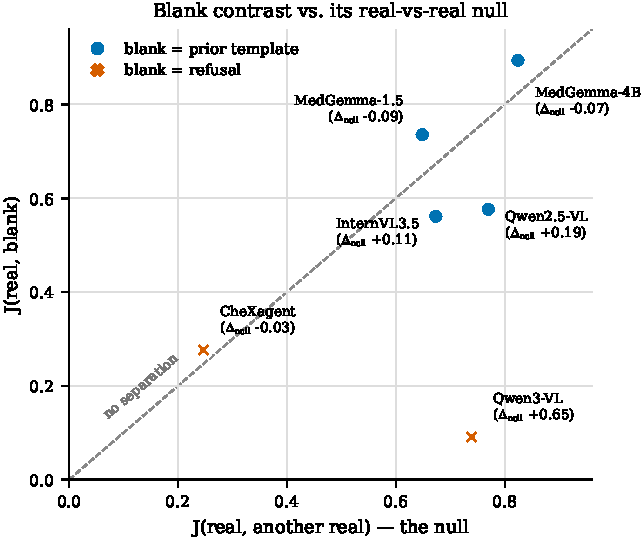
\includegraphics[width=0.62\textwidth]{figures/fig05_blank_null.pdf}
\caption{空白对照与其自身零模型。对角线上的点没有分离；对角线以下的点比随机真实报告更不同。拒答（叉号）远在对角线下方，但它测量的是缺失检测，不是证据提取。}
\label{fig:null}
\end{figure}

\subsection{精度改变输出体制，而不只是权重}
\label{sec:results-precision}

\begin{table}[t]
\centering
\small
\caption{同一模型、同一设计、同一数据——只有精度改变。VRS（视觉依赖分数）为真实图像与空白图像之间的平均绝对概率差（概率空间对照，不是文本相似度）。}
\label{tab:precision}
\begin{tabular}{lrrrrr}
\toprule
模型 & VRS 4-bit & VRS bf16 & 标记率（真实） & 标记率（空白） & 空白 \texttt{no\_finding} 阳性 \\
\midrule
MedGemma-1.5 & 0.129 & 0.284 & \textbf{0.13\% $\rightarrow$ 99.07\%} & 100\% $\rightarrow$ 100\% & \textbf{0\% $\rightarrow$ 100\%} \\
MedGemma-4B & 0.339 & 0.296 & 0\% $\rightarrow$ 0\% & 0\% $\rightarrow$ 0\% & 100\% $\rightarrow$ 100\% \\
Qwen2.5-VL & 0.003 & 0.015 & --- & --- & --- \\
\bottomrule
\end{tabular}
\end{table}

表~\ref{tab:precision} 固定模型、设计、数据与所有提示，只改变精度。MedGemma-1.5 是唯一发生体制切换的模型，其依赖``跨层''（0.129 与 Qwen3-VL 的 0.165 同层；0.284 与 MedGemma-4B 的 0.296 同层）。对照模型没有体制切换：两种精度下标记率均为 0，空白回答本来就在两种精度下都为 \texttt{no\_finding} 阳性；VRS 变化很小且方向相反（0.87 倍）。因此，对精度的测得依赖为 \textbf{0.87--5.22 倍，且方向并不普遍}；但跨层案例是真实的，会破坏任何混合精度排行榜。

\subsection{标签级退化层级在 NIH 上具有模型不变性}
\label{sec:results-labels}

在四个可读模型上，重度退化后按发现排序的召回保持率在原始秩上一致：两两 Spearman \textbf{0.657--0.857}，Kendall 0.619--0.786（$n_{\text{标签}}=6$--7）。合并保持率：心脏增大 0.945 $>$ 肺不张 0.877 $>$ 水肿 0.716 $>$ 实变 0.669 $>$ 肺炎 0.629 $>$ 气胸 0.605。气胸均值只使用三个有定义比值的模型；Qwen3-VL 的干净召回为 0，其比值无定义，因此各标签的分母并不固定。两个干净召回接近零的标签（\texttt{pleural\_effusion}、\texttt{no\_finding}）会产生大于 1 的比值，必须排除或报告绝对召回。

患病率是混杂因素，我们选择报告而不是等审稿人发现。保持率与 NIH 患病率跨标签相关（Spearman 0.43--0.71），并且在每个模型中高患病率标签的平均保持率都更高（附录~\ref{app:risk}，表~\ref{tab:hierarchy}）。对患病率做秩残差化后，两两偏 Spearman 为 $-0.69$ 至 $+0.85$，且符号在不同模型对间改变，因此原始一致性不是患病率无关的规律。逐标签患者聚类自助法给出 28 个模型--标签召回变化中有 22 个在 Benjamini--Hochberg $q<0.05$；例外是心脏增大与接近零召回的气胸（附录~\ref{app:risk}，表~\ref{tab:perlabel}）。这是\emph{单一数据集上的模型不变性，且部分受患病率混杂}：与病灶级效应一致，但不是已被证明的数据集不变或患病率无关规律。实际结论是一条候选设计规则——按发现分层报告鲁棒性——而不是``发现身份单独决定退化敏感性''。外部复现之前，不应把它当作可迁移规律。

\subsection{跨数据集判别力坍缩}
\label{sec:results-transfer}

\begin{table}[t]
\centering
\small
\caption{代表性标签上 NIH 与 PadChest 的 AUROC。``no-finding''与``cardiomegaly''两列均按 NIH $\rightarrow$ PadChest 排列。95\% 区间是对目标域的患者聚类自助法。}
\label{tab:transfer}
\begin{tabular}{lrrr}
\toprule
模型 & no-finding & cardiomegaly & $\Delta$CI（心脏增大） \\
\midrule
InternVL3.5 & 0.774 $\rightarrow$ \textbf{0.500} & 0.672 $\rightarrow$ \textbf{0.500} & $[-0.201,-0.141]$ \\
Qwen3-VL & 0.685 $\rightarrow$ \textbf{0.501} & 0.598 $\rightarrow$ \textbf{0.500} & $[-0.122,-0.071]$ \\
MedGemma-4B & 0.524 $\rightarrow$ 0.508 & 0.690 $\rightarrow$ \textbf{0.492} & $[-0.236,-0.154]$ \\
MedGemma-1.5 & 0.499 $\rightarrow$ 0.496 & 0.675 $\rightarrow$ \textbf{0.541} & $[-0.200,-0.061]$ \\
Qwen2.5-VL & 0.508 $\rightarrow$ 0.500 & 0.504 $\rightarrow$ 0.500 & $[-0.011,+0.002]$ \\
CheXagent & 0.504 $\rightarrow$ 0.500 & 无定义（常数；87 个阳性） & --- \\
\bottomrule
\end{tabular}
\end{table}

只有 MedGemma-1.5 的心脏增大 AUROC 保持高于随机（0.541，区间排除 0.5），它也是唯一保持响应性的模型（表~\ref{tab:transfer}）。两个事实一致：只给出一种回答的模型无法对图像排序，而能对图像排序的模型必须给出不止一种回答（图~\ref{fig:transfer}）。这一坍缩不是 VLM 特有的：同一个 DenseNet-121 在 PadChest 上只达到 0.515 宏 AUROC，而在 NIH 上为 0.733（附录~\ref{app:risk} 表~\ref{tab:densenetgrid}），因此在单一医院训练的监督模型同样无法迁移。

该比较同时改变医院来源、病例构成、标签映射与输入几何，因此下降是\emph{跨数据集}效应，而不是孤立的医院效应。共同标签重算（附录~\ref{app:risk}）去掉了结构性缺失的肺炎项，响应性检查去掉了常数输出解释，但这里没有任何设计能把医院偏移与病例构成偏移分开。因此，我们主张数据集层面的判别力坍缩，而不是量化的医院域惩罚。在标签层面，这一层级在域外不可估计：五个无响应模型最多只给出 20 种不同回答，其逐标签 AUROC 落在 0.492--0.536，不构成有意义的排序；而对唯一有响应的模型（MedGemma-1.5），只有心脏增大的区间高于随机（0.541，95\% CI 0.505--0.584；肺不张 0.531，CI 0.464--0.605），其余四个可估计标签为 0.489--0.490（附录~\ref{app:risk}，表~\ref{tab:padlabel}）。NIH 的标签排序不能作为可排序层级迁移到域外；能迁移的是坍缩本身。

\begin{figure}[t]
\centering
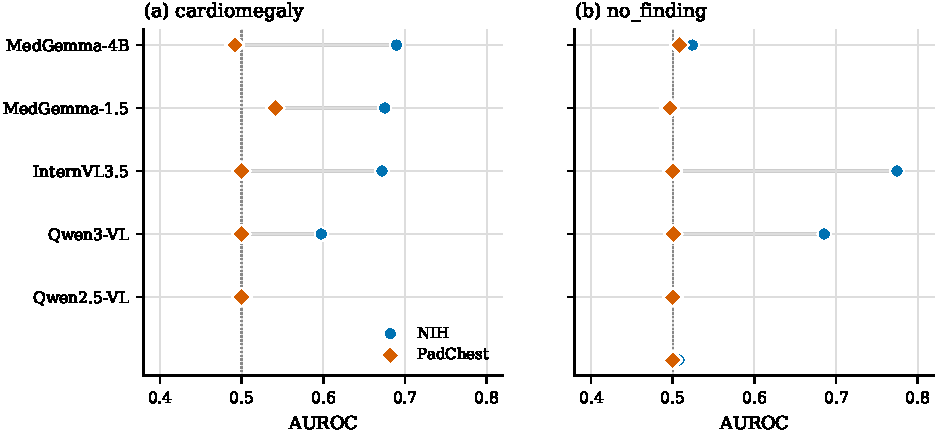
\includegraphics[width=\textwidth]{figures/fig04_transfer.pdf}
\caption{跨数据集迁移（NIH $\rightarrow$ PadChest）。每条线段连接同一模型的 NIH AUROC 与 PadChest AUROC；虚线为随机水平。}
\label{fig:transfer}
\end{figure}

\subsection{报告层：依赖标注器的排序}
\label{sec:results-report}

\begin{table}[t]
\centering
\small
\caption{Open-i 报告层（$n=947$，规则标注器）。}
\label{tab:report}
\begin{tabular}{lrrl}
\toprule
模型 & 漏报 & 幻觉 & 体制 \\
\midrule
CheXagent & \textbf{1,198} & \textbf{113} & 多为``无法判读'' \\
MedGemma-1.5 & 571 & 268 & 保守 \\
Qwen2.5-VL & 302 & 2,128 & 中等漏报、高幻觉 \\
InternVL3.5 & 274 & 2,198 & 同上 \\
MedGemma-4B & 196 & \textbf{3,021} & 低漏报、很高幻觉 \\
Qwen3-VL & \textbf{181} & \textbf{3,508} & 最低漏报、最高幻觉 \\
\bottomrule
\end{tabular}
\end{table}

完整 Open-i 表见附录~\ref{app:protocol} 表~\ref{tab:report}。排序依赖标注器。在规则标注器下，两类错误对六个模型的排序方向相反；在 CheXbert 下（同样 947 例研究），幻觉排序方向保持一致（Spearman 0.71，$n=6$，$p=0.11$），而漏报排序不一致（$-0.49$，$p=0.33$；附录~\ref{app:protocol} 表~\ref{tab:chexbert}）。因此我们不主张普遍的漏报--幻觉权衡：表观权衡是规则标注器的属性，只有幻觉轴稳定到可以作为模型排序报告。

\subsection{选择性预测：没有可用覆盖率}
\label{sec:results-selective}

选择性指标需要模式适配器：矩阵运行器把答案嵌在 \texttt{parsed.findings} 下，而 NIH 依赖文件不带真值，直接把现有选择性预测脚本指向它们会得到零行。本节同时是四个前提的\emph{下游代价}：选择性可信层不可能比它所消费的契约更可识别，其覆盖率在任何风险模型拟合之前就已被契约覆盖所界定。使用适配器后，合规覆盖率在各模型间差异显著：Qwen2.5-VL 100\%、InternVL3.5 99.6\%、MedGemma-1.5 95.2\%、Qwen3-VL 91.7\%、MedGemma-4B 87.9\%、\textbf{CheXagent 18.9\%}。逐单元覆盖普查见附录~\ref{app:protocol} 表~\ref{tab:coverage}。

因此，CheXagent 会依约定产生两个互相矛盾的图像级错误率：跳过无概率标签时为 0.183，把所有非阳性状态视为阴性时为 1.000。两者都不错；它们回答不同问题。它的选择性指标与其他五个不可比，报告时附 \texttt{contract\_coverage} $=0.189$（\texttt{not\_mentioned} $=9{,}486/12{,}016$ 个槽位；只有 9.7\% 的图像八个标签全部确定）。

\begin{table}[t]
\centering
\footnotesize
\setlength{\tabcolsep}{2pt}
\caption{NIH 留出测试集上的选择性预测（$n=1{,}054$ 例研究；8,432 个发现项；427 个患者簇）。``风险''是已回答项中的错误率。AUROC 列为发现级错误检测 AUROC，分别使用单独置信度与置信度加 shift 分数。}
\label{tab:selective}
\begin{tabular}{lrrrrrrr}
\toprule
模型 & 发现错误 & 覆盖@5\% & 覆盖@10\% & 风险@50\% & 风险@80\% & AUC（置信） & +shift \\
\midrule
MedGemma-4B & 0.335 & 0.064 & 0.249 & 0.232 & 0.322 & 0.644 & 0.678 \\
MedGemma-1.5 & 0.323 & 0.093 & 0.332 & 0.173 & 0.270 & 0.737 & 0.737 \\
InternVL3.5 & 0.319 & 0.000 & 0.117 & 0.235 & 0.302 & 0.627 & 0.635 \\
Qwen3-VL & 0.392 & 0.010 & 0.025 & 0.256 & 0.377 & 0.660 & 0.664 \\
Qwen2.5-VL & 0.440 & 0.005 & 0.020 & 0.234 & 0.375 & 0.772 & 0.773 \\
\bottomrule
\end{tabular}
\end{table}

图像级错误被上限主导：每例 NIH 评估研究都至少在一个八标签上为阳性（92\% 至少有一个疾病标签，其余仅为 no-finding），因此全阴预测器的错误率为 0，0.94--0.97 是构成导致的上界伪影。发现级才是可解释的层级（表~\ref{tab:selective}）。在该层级，把 shift 分数加入置信度最多使 AUROC 变化 $+0.034$（MedGemma-4B 0.644$\rightarrow$0.678，InternVL3.5 0.627$\rightarrow$0.635，Qwen3-VL 0.660$\rightarrow$0.664，Qwen2.5-VL 0.772$\rightarrow$0.773），对 MedGemma-1.5 没有影响（0.737$\rightarrow$0.737）；加入图像依赖使两个 MedGemma 模型分别提高 $+0.033$ 与 $+0.006$。因此，排序接近单独置信度已经提供的水平；同时，在 5\% 风险预算下没有模型超过 9.3\% 覆盖率。三动作策略在图像级从不接受（接受率 0.000）。在发现级，它对五个可比模型接受 17--41\% 的条目（CheXagent 在其 18.9\% 契约覆盖下为 12--17\%），但接受项的误差率为 5.7--21.7\%，在每个单元都高于 5\% 预算。因此，它是在唯一能行动的层级上未通过预算，而不是通过拒绝行动来``通过''。

完整风险--覆盖曲线（附录~\ref{app:risk}，图~\ref{fig:risk}）说明 5\% 负结果不是某个阈值的伪影。在 5\% 覆盖率处，风险已达 0.043--0.154；到 10\% 覆盖率时，每个模型都超过 5\% 预算。10\% 预算下的覆盖率为 0.020--0.332；50\% 与 80\% 覆盖率处的风险分别为 0.173--0.256 与 0.270--0.377。该策略在 5\% 下从未达到可用工作点；它在临床认可的 10--20\% 预算下是否可用，是部署决策，而不是本文的主张。

\subsection{受控复现实验}
\label{sec:results-round2}

既有文献留下三个决定上述结论可外推程度的问题：有监督模型是否也会停在随机水平；schema 结果是否只是某一个检查点的习惯；第二个推理模型是否显示同样的轴。本节用预先部署的对照回答这三个问题，并针对 schema 结果检验第四个问题——跨家族的一般性；其余跨家族主张仍未解决，并如实标注。

\subsubsection{监督基线并不处于随机水平}
\label{sec:results-baseline}

我们用 ImageNet 初始化训练 DenseNet-121~\citep{huang2017densely}：$224$\,px、类别加权 BCE、AdamW、固定八个 epoch，不做早停、不做基于测试集的选择。它只见过 3,871 张 \texttt{internal\_train} 图像，与 1,506 例评测研究没有任何患者重叠。在同样的七个病理标签上，它取得\textbf{宏 AUROC 0.733}（95\% 患者聚类自助法区间 0.718--0.749，725 名患者，1,000 次重采样；逐标签 0.620--0.805；表~\ref{tab:baseline}），在其自身 1,352 例患者不重叠的 \texttt{internal\_test} 划分上为 0.724（VLM 评测使用该划分中的 1,054 例子集；第~\ref{sec:protocol} 节）。

\begin{table}[t]
\centering
\small
\caption{干净 NIH 七个病理标签的宏 AUROC（$n=1{,}506$）。基线只用 3,871 张无患者重叠的图像训练；六个 VLM 即表~\ref{tab:clean} 的矩阵。}
\label{tab:baseline}
\begin{tabular}{lrr}
\toprule
模型 & 宏 AUROC & 家族 \\
\midrule
\textbf{DenseNet-121（监督）} & \textbf{0.7329} & CNN，本文训练 \\
MedGemma-4B & 0.6270 & 医学 VLM \\
InternVL3.5-8B & 0.6066 & 通用 VLM \\
MedGemma-1.5 & 0.5852 & 医学 VLM \\
Qwen3-VL-8B & 0.5455 & 通用 VLM \\
Qwen2.5-VL-7B & 0.5013 & 通用 VLM \\
CheXagent-8B & 0.5001 & 胸片专用 \\
\bottomrule
\end{tabular}
\end{table}

因此，这些标签从这些图像上是可学的，水平 0.73，而训练集只有 3,871 张——不到公开训练划分 86,524 张的 5\%。``没有可用判别力''说的是模型，不是任务或单纯的标签噪声。基线也给出反方向的界：0.73 并非临床级，故本文的负结果针对的是\emph{测量可识别性}，而不是胸片分类本身不可能。

\subsubsection{schema 依赖性在第二个医学模型上复现，但映射不同}
\label{sec:results-schema2}

我们在 MedGemma-1.5 上重做五套 schema 扫描（15,060 次调用）。核心结果复现：在空白图像上，\textbf{五套 schema 的病理召回全部为 0.000}，而真实图像上为 0.493--0.614（表~\ref{tab:r2schema}）。没有任何措辞能制造图像依赖。

\emph{未}复现的是每套 schema 落入哪种失效形态。MedGemma-4B 有两种（自信判正常，或被迫弃权）；MedGemma-1.5 出现三种：自信判正常（v0、v1、v3 的空白回答中 \texttt{no\_finding} 阳性率 100\%）、\emph{契约坍缩}（v2 仍给标签但在 99.9\% 的空白回答中丢掉概率对象）、以及拒绝断言（v4 在 100\% 的空白回答中判 \texttt{no\_finding} 阴性，并同样契约坍缩）。真实图像召回最高的是 v4（0.614，比 v0 高 6.3\,\pp{}），而它的空白召回仍为 0.000：提示词移动的是工作点，不是模型获取证据的能力。

正确的表述因此比第~\ref{sec:results-schema} 节的``契约决定捷径的形式''更窄：契约与模型\emph{共同}决定形式，而且这一联合映射不可跨检查点迁移。可迁移的是对基准真正重要的不变性：真实图像召回与空白图像行为由不同因素决定，因此任何 schema 都不能只靠其中之一来验证。

\subsubsection{空白图像结果跨模型家族成立；契约签名不成立}
\label{sec:results-xfamily}

为区分 MedGemma 习惯与契约效应，我们在 Qwen3-VL-8B（不同家族的通用模型）上重做扫描（表~\ref{tab:r2xfamily}）。空白图像结果精确复现：三套 schema 下空白图像的病理召回均为 \textbf{0.000}，真实图像为 0.258--0.306。可观察签名没有复现：Qwen3 的 v0 是自信正常（空白回答中 \texttt{no\_finding} 阳性 100\%），但八个请求概率只给出一个，概率完整度空白 12.5\%、真实 47.1\%；v1 保持同样的自信正常答案，同时把完整度恢复到 100\% 与 95.2\%；v4 拒绝正常断言（空白中 \texttt{no\_finding} 阳性 0\%），并在 98\% 的真实回答中契约坍缩。两个模型出现相同的三种失效形态，但 variant 到形态的映射不同。因此契约覆盖是 schema 的属性，而不是模型的属性；空白图像依赖则同时是二者的属性。

\begin{table}[t]
\centering
\footnotesize
\setlength{\tabcolsep}{3.5pt}
\caption{Qwen3-VL-8B 上的跨家族 schema 扫描（每格 $n=1{,}506$）。三套 schema 下空白图像的病理召回均为 0.000，因此空白依赖不是 MedGemma 的习惯。可观察签名不同：v0 自信正常但只给一个概率，v1 自信正常且契约完整，v4 拒绝正常断言并契约坍缩。}
\label{tab:r2xfamily}
\begin{tabular}{lrrrrrr}
\toprule
方案 & 真实召回 & 空白召回 & 空白 \texttt{no\_finding} 阳性 & 违约（真实/空白） & 完整度（真实/空白） \\
\midrule
v0 简单 & 0.306 & \textbf{0.000} & 1.000 & 0.611 / 1.000 & 0.471 / 0.125 \\
v1 逐标签二分类 & 0.258 & \textbf{0.000} & 1.000 & 0.054 / 0.000 & 0.952 / 1.000 \\
v4 正常性施压 & 0.263 & \textbf{0.000} & 0.000 & 0.983 / 1.000 & 0.849 / 0.875 \\
\bottomrule
\end{tabular}
\end{table}

\subsubsection{措辞不是机制，但它决定空白图像上的答案}
\label{sec:results-paraphrase}

我们在 MedGemma-4B 上对 v0 契约做了两个改写版本（标签集合、状态规则、JSON 结构完全一致），对真实与空白图像各跑一遍（6,024 次调用）。真实图像上，发现级答案可复现：与 v0 基线的一致率为 90.9\% 与 91.4\%，Cohen's $\kappa$ 为 0.624 与 0.642。schema 结论不是单一措辞的产物。

空白图像上，两个改写版本与基线只在一个标签上分歧。v0 在 100\% 的空白回答中判 \texttt{no\_finding} 阳性；p2 相同（一致率 1.000）；p1 在 100\% 中判阴性（一致率 0.000）。病理标签在三者之间完全一致（全阴性，一致率 1.000）。也就是说，空白图像上的答案由措辞决定、不含任何图像信息——这正是为什么零模型前提需要一个空白对照\emph{并且}一个措辞对照，而不是二者之一。

该对照也在 Qwen3-VL 上运行（表~\ref{tab:r2para}）。两个改写版本都复现真实图像答案（p1 一致率 93.1\%，$\kappa$ 0.723；p2 90.3\%，$\kappa$ 0.701），但都不翻转空白图像答案：与 v0 的空白一致率均为 1.000，而 p1 会把 MedGemma-4B 的空白答案完全翻转。因此措辞设定的是模型特定的先验：同一改写把 MedGemma 的空白答案变负，却让 Qwen3 的自信正常答案保持不变。

\subsubsection{第二个推理模型：同一工作点，新的失效模式}
\label{sec:results-second}

Qwen3-VL-8B-Thinking 具有原生推理通道（chat 模板预填 \texttt{<think>}，模型在回答前闭合它），因此可察觉性轴第一次能在第二个模型上读出。我们在全部 1,506 例研究上跑了七个格子（clean 加六个 severe）。只有闭合推理块\emph{并且}其后能解析出 JSON 的回复才算可用答案，其余作为实测结果保留（表~\ref{tab:r2recon}）。

\textbf{覆盖率本身是可测量，且随退化下降。} 在 5,120 token 预算下，10,542 个格子中有 9,381 个给出可用答案（89.0\%）；对 40 个格子的 8,192 token 抽样再补 20 个（最终 89.2\%）。覆盖率为 clean 92.6\%、分辨率 severe 80.9\%、亮度 severe 84.3\%（表~\ref{tab:r2think}）。失败并非``加大预算即可消除的截断''：仍然失败的回复中位长度在 2,560 上限时为 9.8k 字符、3,584 时为 13.5k、5,120 时为 19.3k，在 8,192 的 40 格随机抽样中为 28.1k——它们会撑满给它的任何预算；8,192 抽样只能救回 50\%（表~\ref{tab:r2budget}）。不终止是模型行为，我们按行为报告。这是 overthinking 文献在视觉语言模型上的对应：超过某个点，追加推理 token 的边际价值为负，并可能放弃模型本来已经得到的答案~\citep{wu2026whenmore,zhou2026overthinking}；被截断的推理链可能比不推理更糟~\citep{su2026broken}。这里的失效更严重——回复根本无法解析——因此预算曲线是该模型的测量属性，而不只是成本。

\begin{table}[t]
\centering
\footnotesize
\setlength{\tabcolsep}{3.5pt}
\caption{第二个推理模型，severe 格（每格 $n=1{,}506$）。覆盖率为 5,120 token 预算下给出可用答案的研究比例；$\Delta$ 召回为与 clean 在同一批共同作答研究上的配对差（noise $n=1{,}238$；resolution $n=1{,}132$）。AUROC 为七个病理标签的宏平均；阳性率为被判阳性的病理槽位比例。}
\label{tab:r2think}
\begin{tabular}{lrrrrr}
\toprule
格子 & 覆盖率 & 链长(k) & 阳性率 & 宏 AUROC & $\Delta$ 召回 \\
\midrule
clean & 0.926 & 8.73 & 0.250 & 0.547 & --- \\
blur & 0.932 & 8.84 & 0.189 & 0.547 & $-5.5$\,\pp{} \\
brightness & 0.843 & 9.56 & 0.213 & 0.550 & $-5.1$\,\pp{} \\
contrast & 0.924 & 8.99 & 0.280 & 0.545 & $+2.2$\,\pp{} \\
JPEG & 0.923 & 9.37 & 0.240 & 0.537 & $-1.8$\,\pp{} \\
noise & 0.885 & 9.06 & 0.173 & 0.527 & $\mathbf{-10.3}$\,\pp{} \\
resolution & \textbf{0.809} & \textbf{10.22} & \textbf{0.125} & 0.549 & $\mathbf{-13.2}$\,\pp{} \\
\bottomrule
\end{tabular}
\end{table}

\textbf{工作点机制复现，方向相反。} 分辨率损失下阳性率由 0.250 降至 0.125，\texttt{no\_finding} 阳性率由 0.283 升至 0.450，而宏 AUROC 在各格中稳定在 0.527--0.550。由于覆盖率同时下降，我们在配对子集（两格都给出可用答案的研究）上重算该比率：0.250 $\rightarrow$ 0.128，即这一移动不是覆盖率伪影（附录~\ref{app:round2}，表~\ref{tab:r2posrate}）。模型并未丢失排序信息——它本来就没有——它把工作点移向``正常''。这与第~\ref{sec:results-op} 节互为镜像：那里干净阳性率高的模型在退化下上移、召回上升；这里干净阳性率仅 25\% 的模型下移、召回下降。二者都是工作点移动，都不是鲁棒性变化。

逐标签看，配对损失经聚类自助法与多重比较控制后依然显著：胸腔积液 $-8.8$ $[-11.9,-5.8]$\,\pp{}、肺炎 $-11.0$ $[-16.4,-5.5]$\,\pp{}（$q<0.001$）、心影增大 $-6.0$ $[-9.9,-1.9]$\,\pp{}（$q=0.014$）、肺不张 $-2.2$ 与肺水肿 $-4.2$\,\pp{}（$q=0.053$），实变与气胸不显著（表~\ref{tab:r2label}）。

\textbf{轴对通用，象限不通用。} 以覆盖率损失作为该模型的可察觉性读数、以配对召回变化作为损伤，两者再次可分离（与 $|\Delta|$ 的 Spearman 0.49，$p=0.33$；与带符号 $\Delta$ 的为 $-0.54$，$p=0.27$；$n=6$）。在同一 $|\Delta|$ 定义下，MedGemma-1.5 的标记--损伤相关也是 0.49，但六个点使两个估计都无法与零区分：我们主张同一\emph{方向}，而不是共同斜率。噪声换位了：对 MedGemma-1.5，噪声是静默退化（标记率 0.46\%，倒数第二低）而损伤与分辨率损失相当；对 Qwen3-VL-Thinking，噪声是响亮的（覆盖率损失 11.5\%，第三高），并造成 10.3\,\pp{} 的召回损失。\emph{静默失效是监测通道的属性，而不是退化的属性}：盯着推理是否终止的通道能看见噪声，盯着某个特定标记词的通道看不见。

这也解释了为什么第二个模型没有复现反转 3 的正号。该反转需要阳性率有上行空间；一个只把 25\% 槽位判阳的模型几乎没有空间，退化只能把它往下推。按第四前提报告工作点，正是使两个模型可比的原因。


\subsection{核心判断的敏感性}
\label{sec:sensitivity}

三个最关键阈值已在全范围扫描（附录~\ref{app:risk}，\url{scripts/81_sensitivity_analyses.py}）。19 格网格本身是探索性的剂量--响应设计：逐格对照是描述性的，未跨格子做多重比较校正，也不对其附加族错误率主张。确证性的量是第~\ref{sec:preconditions}~节声明的四个审计统计量，以及第~\ref{sec:results-round2} 节的复现实验。

\textbf{(i) 坍缩规则。}把众数占比阈值在 $0.30$--$0.80$ 上变化、唯一回答数上限在 $1$--$20$ 上变化，只会改变哪些边际单元被标记（表~\ref{tab:sweep}），不改变跨数据集结论：在 PadChest 上，六个模型中有五个在 $0.40$ 至 $0.80$ 的每个阈值下都坍缩；在最宽松的 $0.30$ 切点，给出 329 种不同回答的 MedGemma-1.5 也被标记，因此六个全部坍缩。域内被标记集合随阈值升高而缩小（Qwen3-VL 在 $0.60$ 退出，CheXagent 在 $0.70$ 退出）；在 Open-i 上，MedGemma-4B 在低于 $0.70$ 时被标记，$0.30$ 时 Qwen3-VL 也被标记。本文没有任何主张依赖这些边际单元。

\textbf{(ii) 真实图像间零模型的配对。}对 Open-i，在 (a) 随机图像对与 (b) 参考报告长度匹配对下重算真实图像间 Jaccard。零模型最多变化 $0.020$（表~\ref{tab:sens}；MedGemma-4B：0.824 对 0.844），所有分离保持符号与量级：Qwen3-VL 仍远高于其零模型（$+0.648$ 对 $+0.643$），Qwen2.5-VL 保持 $+0.19$，MedGemma-4B 与 MedGemma-1.5 保持负值（$-0.070$ 与 $-0.087$）。``空白是另一种模板，而不是证据''这一解读对配对规则稳健。

\textbf{(iii) 多重比较校正下的迁移区间。}表~\ref{tab:transfer} 报告的跨数据集 $\Delta$AUROC 区间是单次两两 95\% 区间。我们对该家族的 16 个可估计模型--标签单元做 Bonferroni 校正（$z=2.955$）。四个大损失全部存活：InternVL3.5 \texttt{cardiomegaly}（校正后上界 $-0.127$）、InternVL3.5 \texttt{consolidation}（$-0.048$）、MedGemma-4B \texttt{cardiomegaly}（$-0.136$）、MedGemma-1.5 \texttt{cardiomegaly}（$-0.030$）仍严格低于零。两个边缘差值（MedGemma-4B 与 MedGemma-1.5 的 \texttt{no\_finding}）变为不显著，一些本来就接近随机的实变与心脏增大小单元也是如此；四个大损失不受影响。``迁移坍缩''这一主张稳健；少数接近零的单元则不是。

\textbf{(iv) 工作点构成。}InternVL3.5 对比度/重度单元在单张图像层面分解（附录~\ref{app:risk}）。在转移最多的三个发现中，``召回增益''完全来自干净条件下为阴性的图像上的新真阳性（$gt\_pos$：分别获得 $+43$、$+30$、$+50$，丢失 $10$、$3$、$1$），而此前正确的阴性状态以相当的比例翻转为假阳性（$gt\_neg$：$+36$、$+59$、$+69$）。净假阳性上升（表~\ref{tab:op}）。这与广泛的工作点移动一致，而不是有针对性地找回丢失发现；它本身不能识别阈值机制。

\begin{figure}[t]
\centering
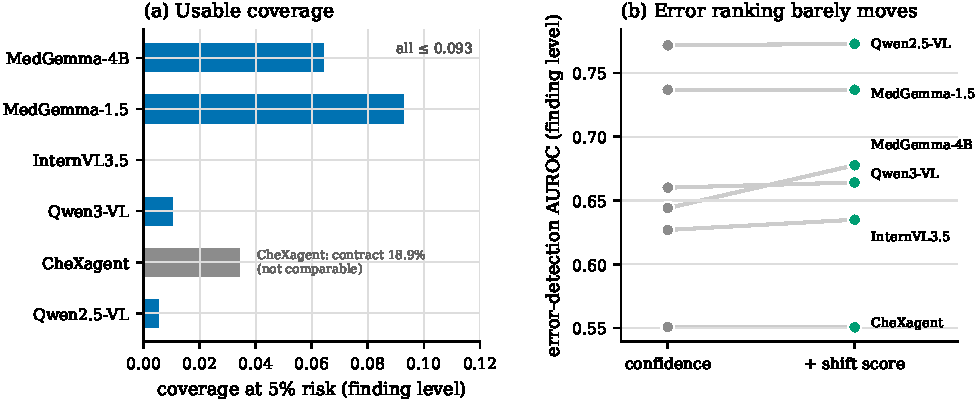
\includegraphics[width=\textwidth]{figures/fig06_selective.pdf}
\caption{(a) 5\% 风险预算下的可用覆盖率最多为 0.093；CheXagent 的柱为灰色，因为其契约只覆盖 18.9\% 的槽位。(b) 在发现级，同样的信号只使错误排序发生边际变化。排序能力与决策有用性是两件事。}
\label{fig:selective}
\end{figure}

\begin{figure}[t]
\centering
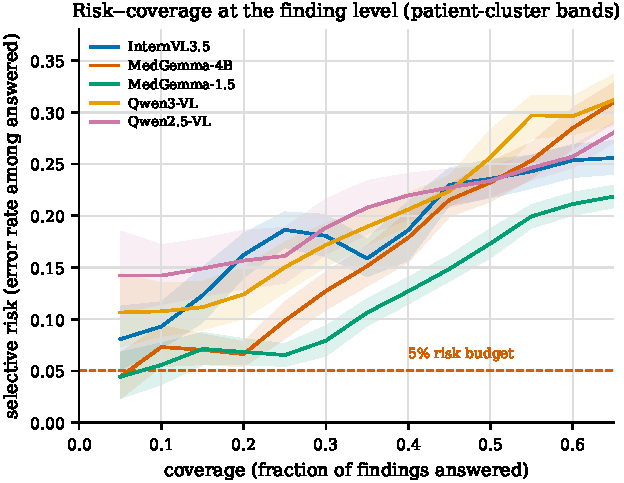
\includegraphics[width=0.62\textwidth]{figures/fig07_risk_coverage.pdf}
\caption{发现级风险--覆盖曲线，含患者聚类自助法带（1,000 次重采样）。在 5\% 覆盖率处风险为 0.043--0.154；到 10\% 覆盖率时每个模型都超过 5\% 预算；5\% 预算最多允许 0.093 覆盖率，10\% 预算允许 0.02--0.33，具体取决于模型。}
\label{fig:risk}
\end{figure}
